\subsection{Finite Difference Time Domain}
Finite Difference Time Domain (FDTD) is a very computationally intensive way to simulate the propagation of electromagnetic radiation.  It solves full on Maxwell's equations in time domain making no assumptions.  This approach has only been possible in the last few years with the increase in computing power.

Food for thought: Before using FDTD, you should be aware that in many cases when simulating a device, using FDTD is like using a sledge hammer to crack a nut.  For example when simulating a standard solar cell, one could use FDTD, this would involve simulating a wave front entering the cell through the top contact in time domain and waiting until the optical field reaches steady state then calculating how much light is being absorbed. This would require thousands of time domain simulation steps per wavelength.  However usually one is not interested in the time evolution of light in a solar cell as sunlight varies very slowly indeed, so one is better off not using a steady state method but other methods which assume light has already reached steady state, such as the transfer matrix method discussed above.

Never the less, FDTD is an import method, and can be used to design and understand complex devices.

\subsubsection{Running an FDTD simulation}

\begin{figure}[H]
\centering
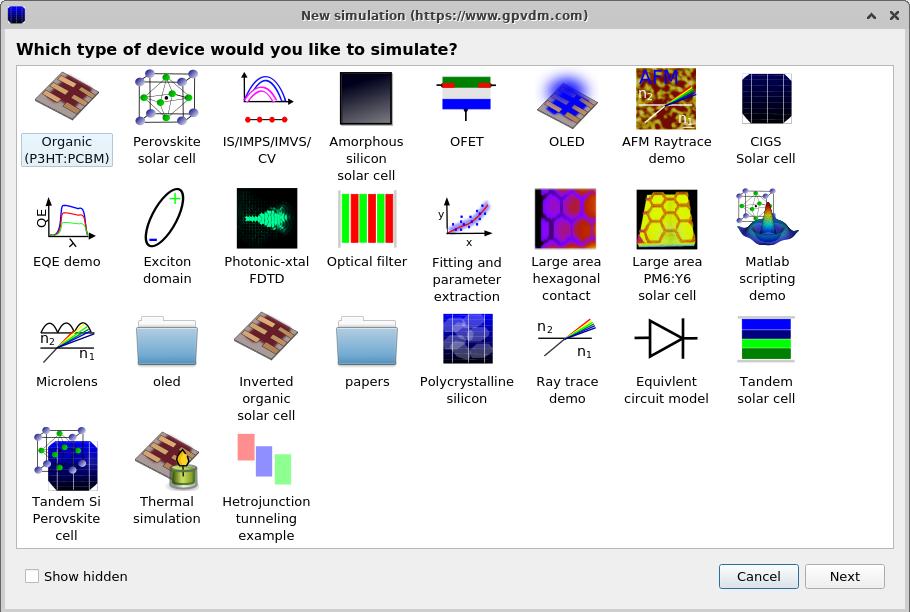
\includegraphics[width=0.7\textwidth]{./images/fdtd_1.png}
\caption{FDTD  }
\label{fig:build}
\end{figure}

\begin{figure}[H]
\centering
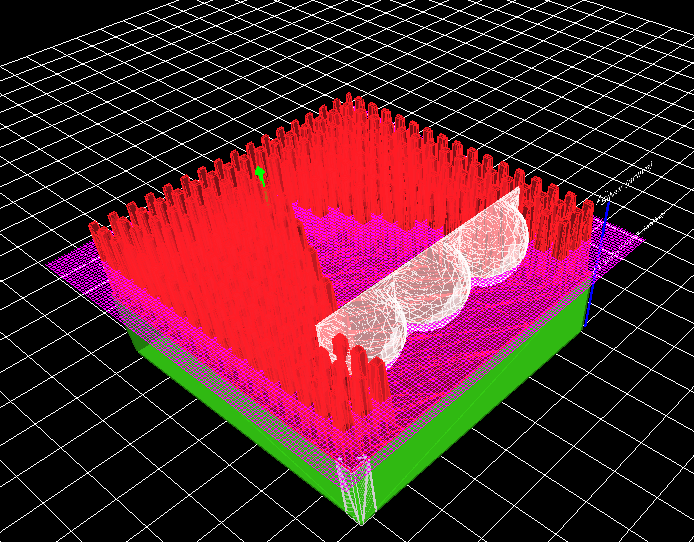
\includegraphics[width=0.7\textwidth]{./images/fdtd_2.png}
\caption{FDTD  }
\label{fig:build}
\end{figure}

\begin{figure}[H]
\centering
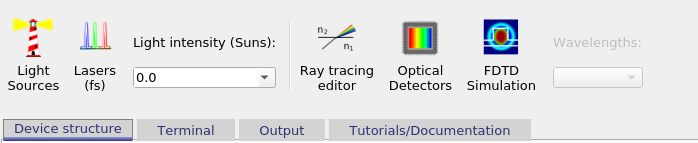
\includegraphics[width=0.7\textwidth]{./images/fdtd_3.png}
\caption{FDTD  }
\label{fig:build}
\end{figure}

\begin{figure}[H]
\centering
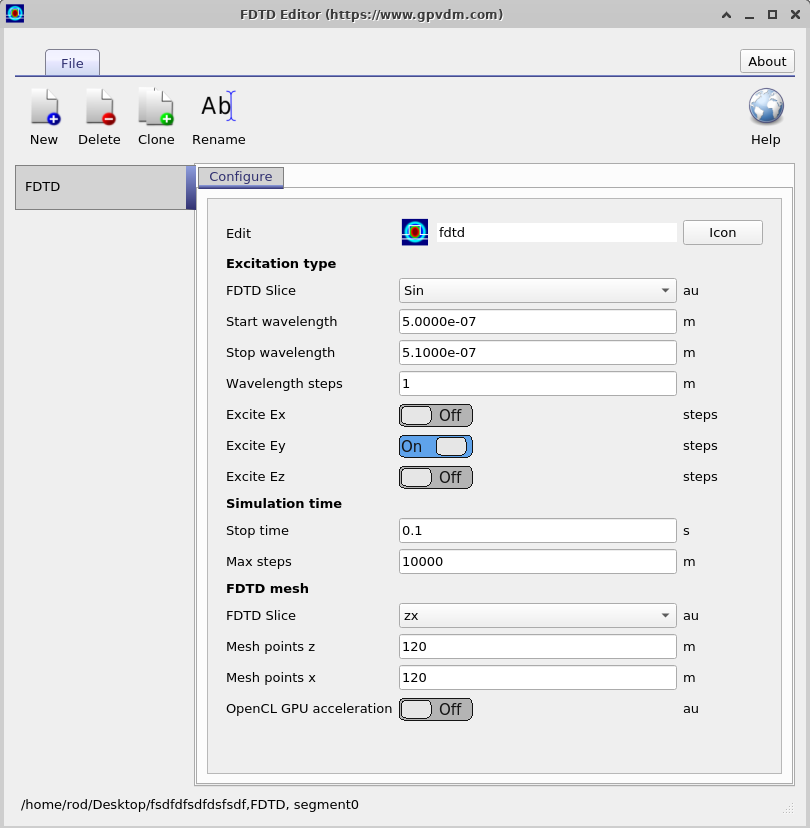
\includegraphics[width=0.7\textwidth]{./images/fdtd_4.png}
\caption{FDTD  }
\label{fig:build}
\end{figure}

\begin{figure}[H]
\centering
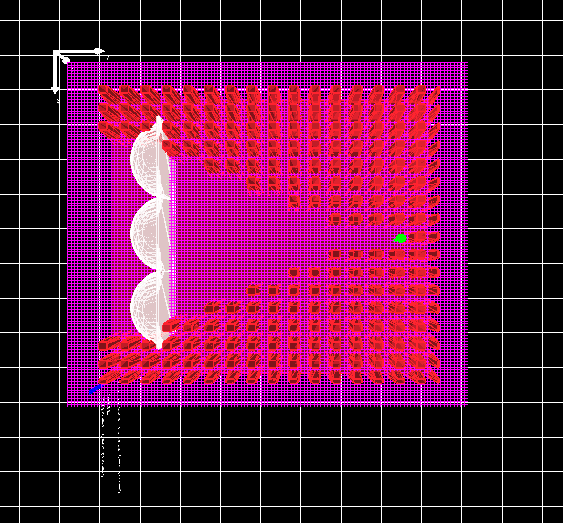
\includegraphics[width=0.7\textwidth]{./images/fdtd_5.png}
\caption{FDTD  }
\label{fig:build}
\end{figure}

\begin{figure}[H]
\centering
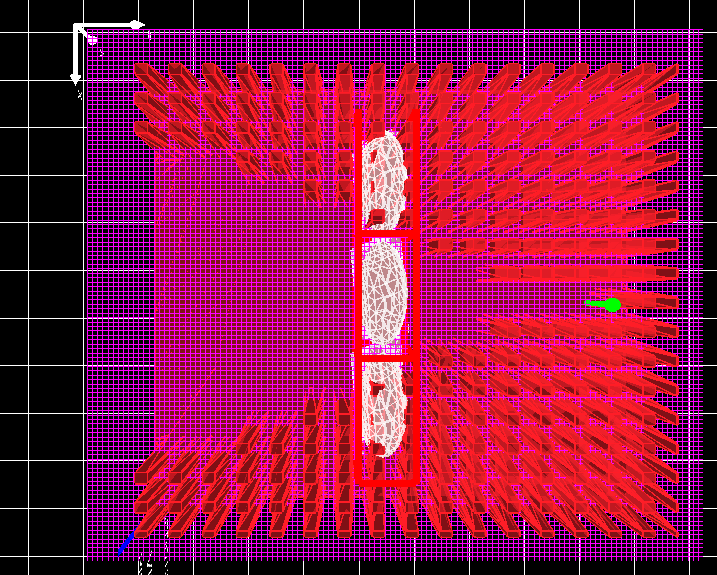
\includegraphics[width=0.7\textwidth]{./images/fdtd_6.png}
\caption{FDTD  }
\label{fig:build}
\end{figure}

\begin{figure}[H]
\centering
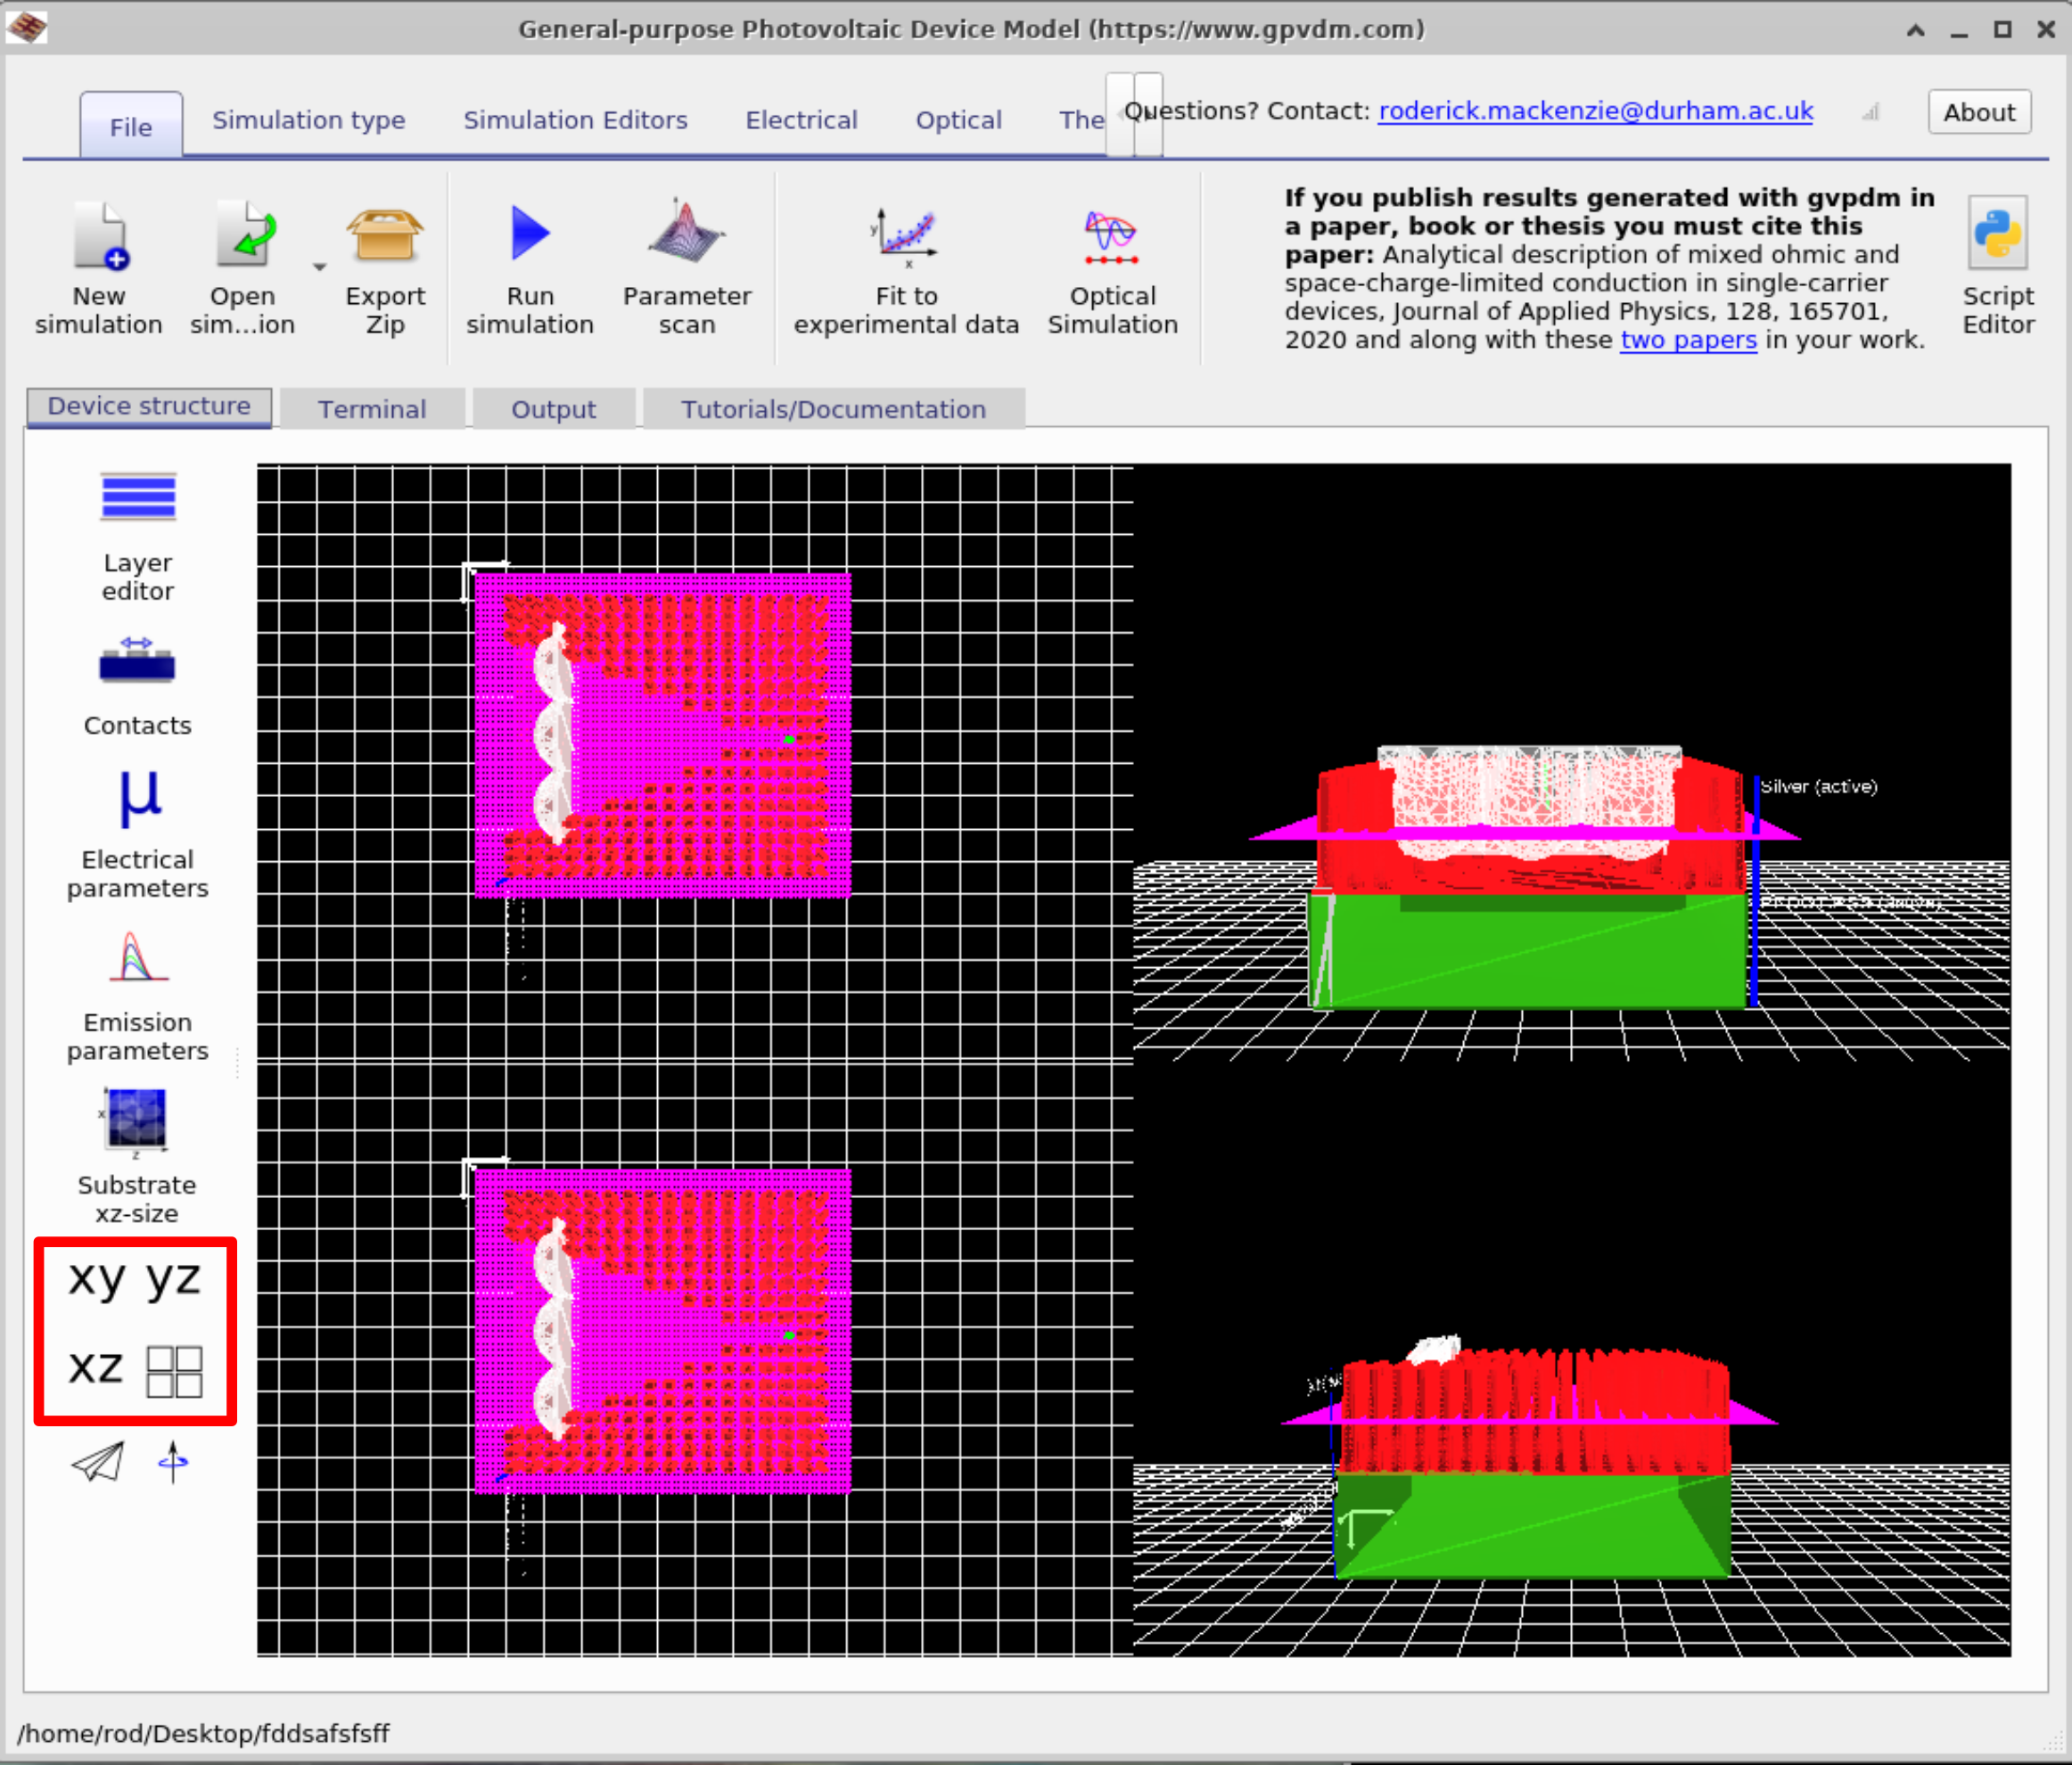
\includegraphics[width=0.7\textwidth]{./images/fdtd_7.png}
\caption{FDTD  }
\label{fig:build}
\end{figure}

\begin{figure}[H]
\centering
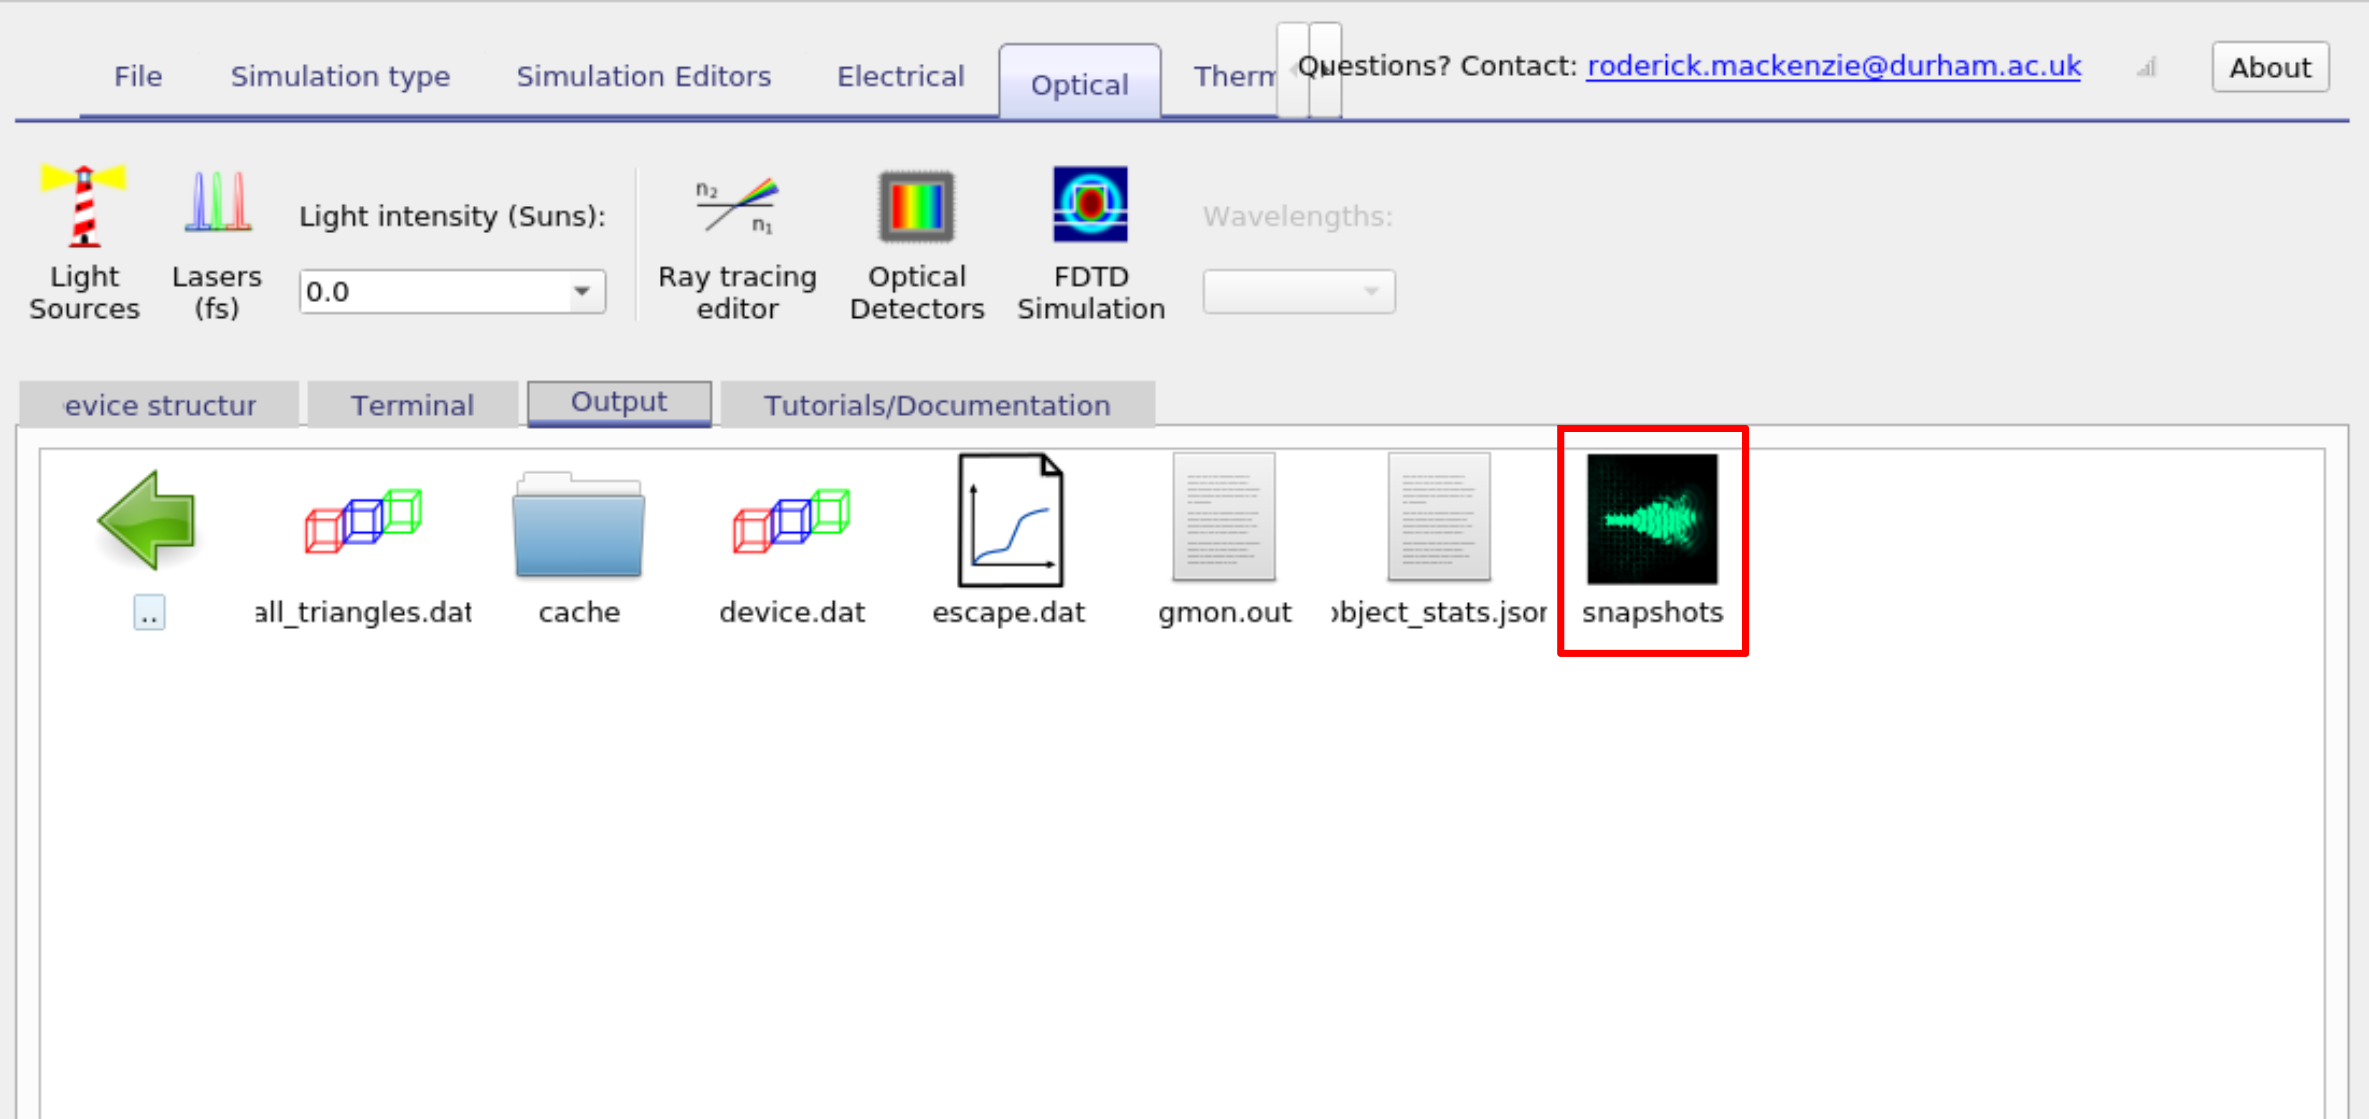
\includegraphics[width=0.7\textwidth]{./images/fdtd_8.png}
\caption{FDTD  }
\label{fig:build}
\end{figure}

\begin{figure}[H]
\centering
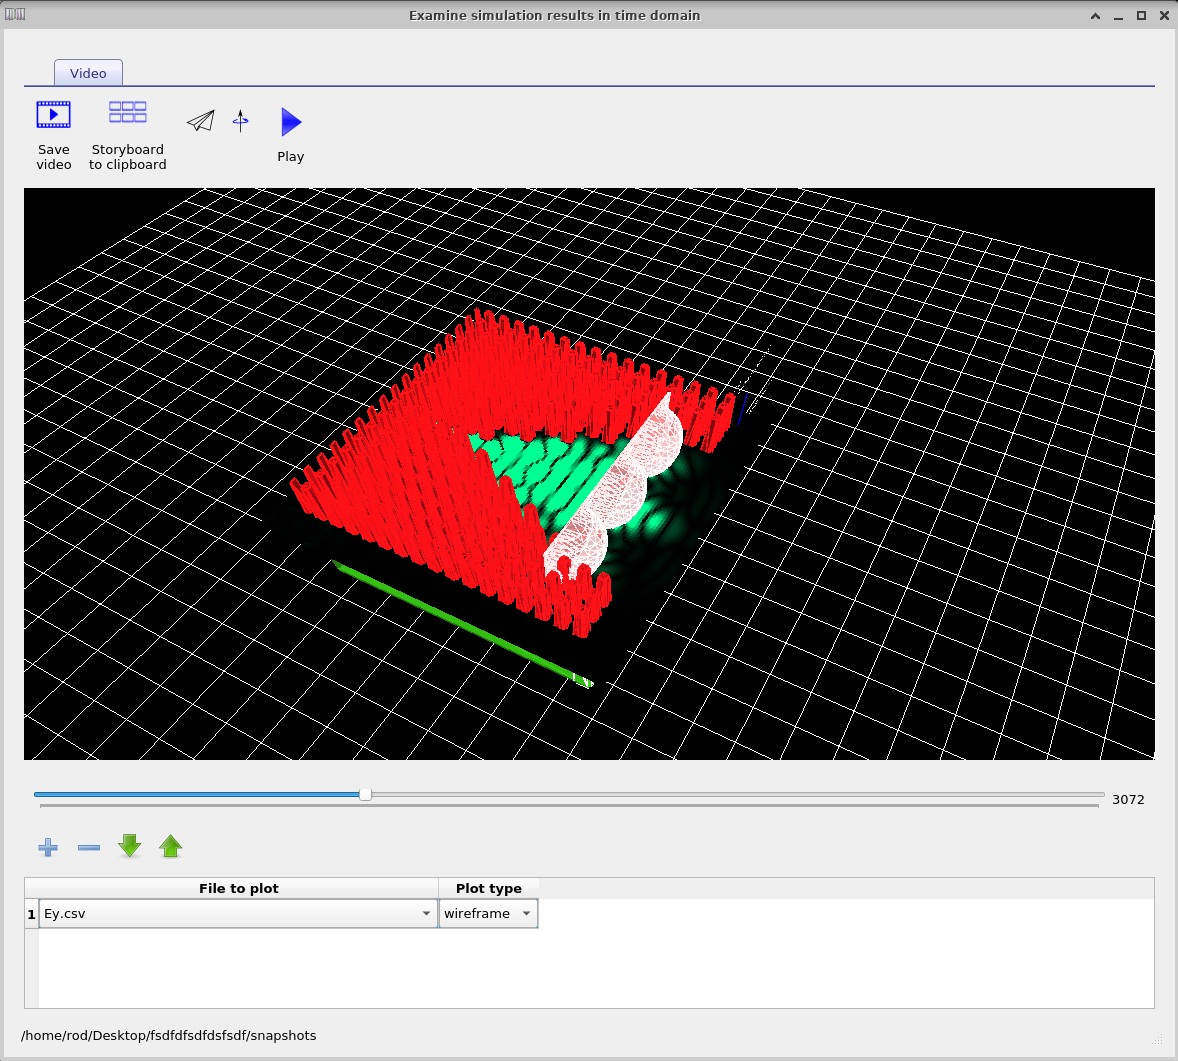
\includegraphics[width=0.7\textwidth]{./images/fdtd_9.png}
\caption{FDTD  }
\label{fig:build}
\end{figure}

\begin{figure}[H]
\centering
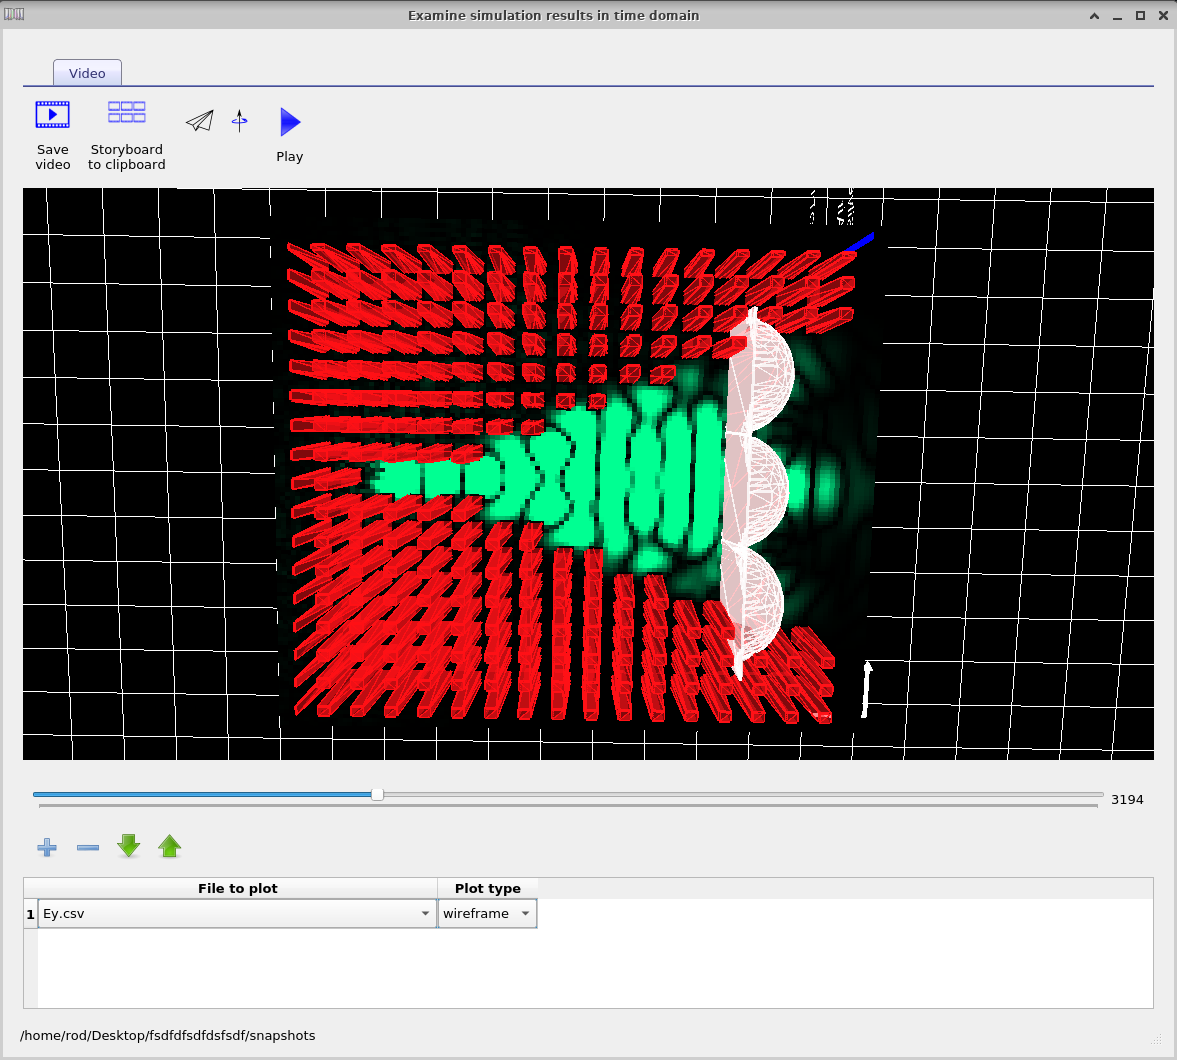
\includegraphics[width=0.7\textwidth]{./images/fdtd_10.png}
\caption{FDTD  }
\label{fig:build}
\end{figure}

\begin{figure}[H]
\centering
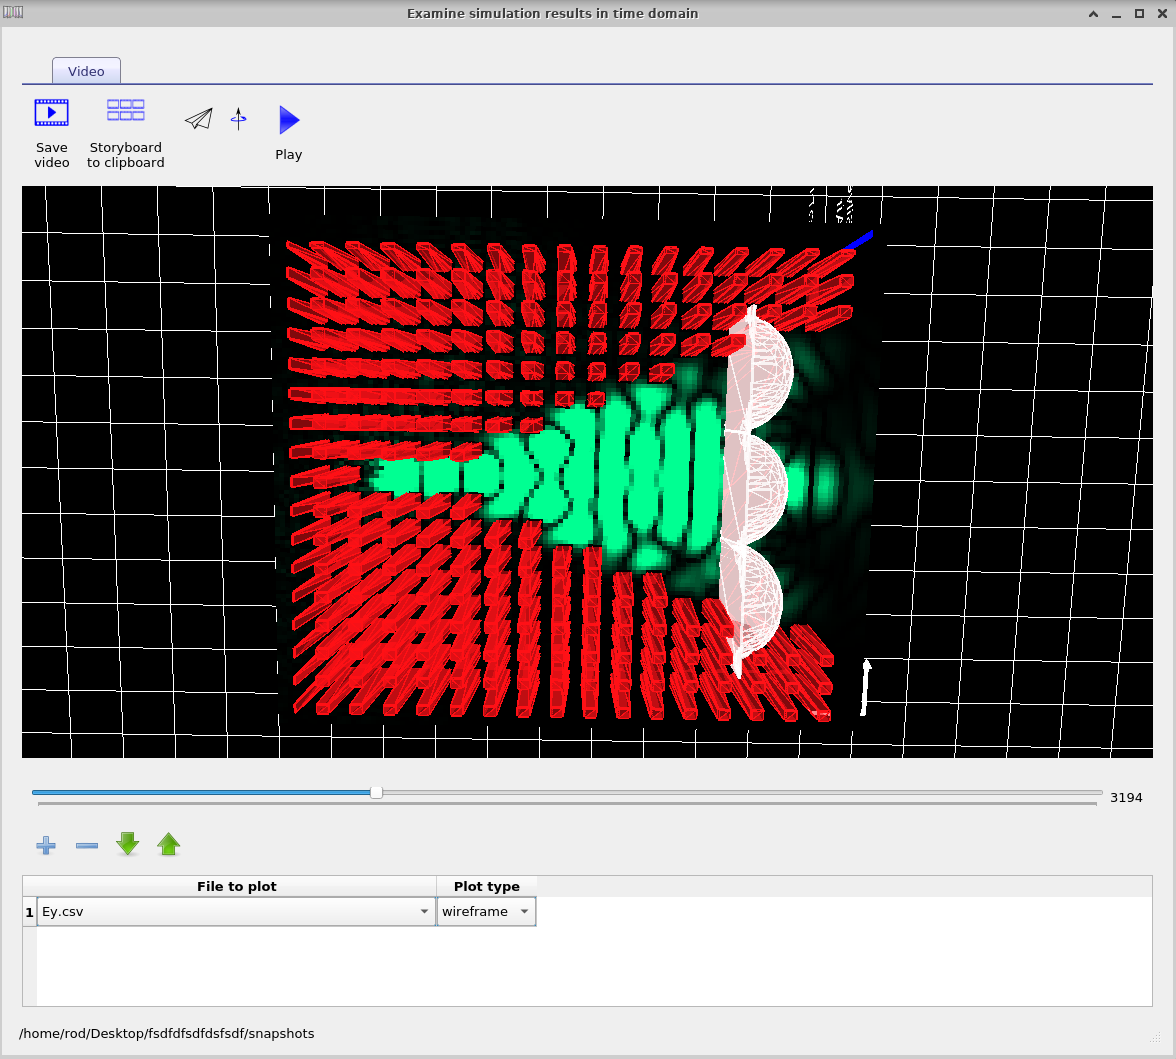
\includegraphics[width=0.7\textwidth]{./images/fdtd_11.png}
\caption{FDTD  }
\label{fig:build}
\end{figure}

\begin{figure}[H]
\centering
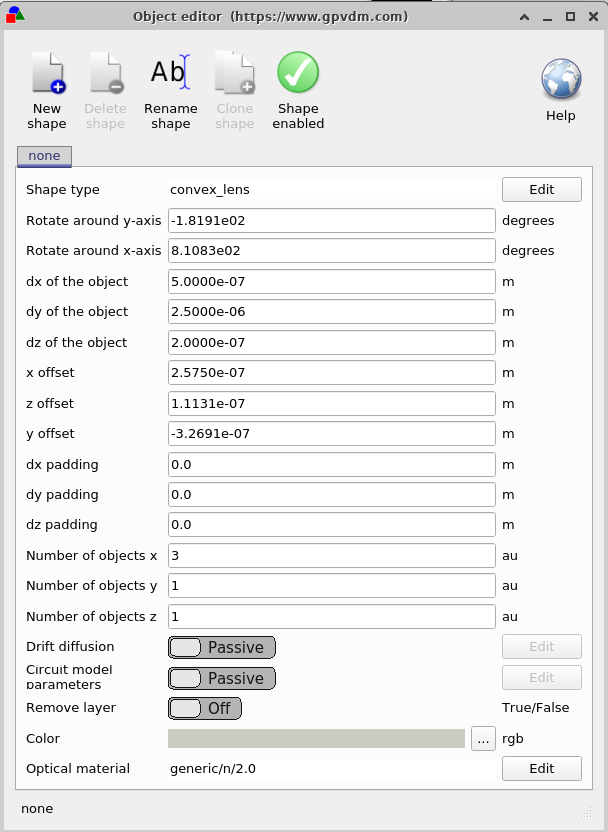
\includegraphics[width=0.7\textwidth]{./images/fdtd_12.png}
\caption{FDTD  }
\label{fig:build}
\end{figure}
\subsubsection{Theoretical background}
References for this section are \cite{FDTD_Schneider}. This section of the manual aims to describe the FDTD code in full with verbose derivations to help understanding/pick up errors.

Ampere’s law is given as  \cite{FDTD_Schneider}
\begin{equation}
\sigma  \boldsymbol{E} + \epsilon \frac{\partial  \boldsymbol{E}}{\partial t} = \nabla \times \boldsymbol{H} =
\begin{vmatrix} \hat{\boldsymbol{x}} & \hat{\boldsymbol{y}} & \hat{\boldsymbol{z}} \\ 
\frac{\partial}{\partial x} & \frac{\partial}{\partial y} & \frac{\partial}{\partial z} \\ 
H_{x} & H_{y} & H_{z}
\end{vmatrix}
\end{equation}


which can be expanded as

\begin{equation}
\sigma  E_{x} + \epsilon \frac{\partial  E_{x}}{\partial t} = \frac{\partial  H_{z}}{\partial y}-\frac{\partial  H_{y}}{\partial z}
\end{equation}

\begin{equation}
\sigma  E_{y} + \epsilon \frac{\partial  E_{y}}{\partial t} = -\frac{\partial  H_{z}}{\partial x}+\frac{\partial  H_{x}}{\partial z}
\end{equation}

\begin{equation}
\sigma  E_{z} + \epsilon \frac{\partial  E_{z}}{\partial t} = \frac{\partial  H_{y}}{\partial x}-\frac{\partial  H_{x}}{\partial y}
\end{equation}


For the case $\frac{\partial}{\partial y}=0$

\begin{equation}
\begin{split}
&\sigma  E_{x} + \epsilon \frac{\partial  E_{x}}{\partial t} =-\frac{\partial  H_{y}}{\partial z}\\
&\sigma  E_{y} + \epsilon \frac{\partial  E_{y}}{\partial t} = -\frac{\partial  H_{z}}{\partial x}+\frac{\partial  H_{x}}{\partial z}\\
&\sigma  E_{z} + \epsilon \frac{\partial  E_{z}}{\partial t} = \frac{\partial  H_{y}}{\partial x}
\end{split}
\end{equation}

for $E_{x}$
\begin{equation}
\begin{split}
&\sigma  E_{x} + \epsilon \frac{\partial  E_{x}}{\partial t} =-\frac{\partial  H_{y}}{\partial z}\\
&\sigma  \frac{E_{x}^{t+1}[]+E_{x}^{t}[]}{2} + \epsilon \frac{E_{x}^{t+1}[]-E_{x}^{t}[]}{\Delta t} = -\frac{H_{y}^{t+\frac{1}{2}}[\frac{1}{2}]-H_{y}^{t+\frac{1}{2}}[-\frac{1}{2}]}{\Delta z}\\
&\sigma  \frac{E_{x}^{t+1}[]}{2} + \epsilon \frac{E_{x}^{t+1}[]}{\Delta t} = -\frac{H_{y}^{t+\frac{1}{2}}[\frac{1}{2}]-H_{y}^{t+\frac{1}{2}}[-\frac{1}{2}]}{\Delta z}-\sigma  \frac{E_{x}^{t}[]}{2}+\epsilon \frac{E_{x}^{t}[]}{\Delta t}\\
&\sigma  \frac{E_{x}^{t+1}[]}{2} + \epsilon \frac{E_{x}^{t+1}[]}{\Delta t} = -\frac{H_{y}^{t+\frac{1}{2}}[\frac{1}{2}]-H_{y}^{t+\frac{1}{2}}[-\frac{1}{2}]}{\Delta z}-\sigma  \frac{E_{x}^{t}[]}{2}+\epsilon \frac{E_{x}^{t}[]}{\Delta t}\\
& \frac{\sigma \Delta t  + 2 \epsilon  }{ 2 \Delta t}E_{x}^{t+1}[] = -\frac{H_{y}^{t+\frac{1}{2}}[\frac{1}{2}]-H_{y}^{t+\frac{1}{2}}[-\frac{1}{2}]}{\Delta z}-\sigma  \frac{E_{x}^{t}[]}{2}+\epsilon \frac{E_{x}^{t}[]}{\Delta t}\\
& E_{x}^{t+1}[] = \left ( -\frac{H_{y}^{t+\frac{1}{2}}[\frac{1}{2}]-H_{y}^{t+\frac{1}{2}}[-\frac{1}{2}]}{\Delta z}-\sigma  \frac{E_{x}^{t}[]}{2}+\epsilon \frac{E_{x}^{t}[]}{\Delta t} \right ) \frac{2 \Delta t}{\sigma \Delta t  + 2 \epsilon}
\end{split}
\end{equation}

for $E_{y}$
\begin{equation}
\begin{split}
&\sigma  E_{y} + \epsilon \frac{\partial  E_{y}}{\partial t} = -\frac{\partial  H_{z}}{\partial x}+\frac{\partial  H_{x}}{\partial z}\\
&\sigma  \frac{E_{y}^{t+1}[]+E_{y}^{t}[]}{2} + \epsilon \frac{E_{y}^{t+1}[]-E_{y}^{t}[]}{\Delta t} = -\frac{H_{z}^{t+\frac{1}{2}}[\frac{1}{2}]-H_{z}^{t+\frac{1}{2}}[-\frac{1}{2}]}{\Delta x}+\frac{H_{x}^{t+\frac{1}{2}}[\frac{1}{2}]-H_{x}^{t+\frac{1}{2}}[-\frac{1}{2}]}{\Delta z}\\
&\sigma  \frac{E_{y}^{t+1}[]}{2} + \epsilon \frac{E_{y}^{t+1}[]}{\Delta t} = -\frac{H_{z}^{t+\frac{1}{2}}[\frac{1}{2}]-H_{z}^{t+\frac{1}{2}}[-\frac{1}{2}]}{\Delta x}+\frac{H_{x}^{t+\frac{1}{2}}[\frac{1}{2}]-H_{x}^{t+\frac{1}{2}}[-\frac{1}{2}]}{\Delta z}-\sigma \frac{E_{y}^{t}[]}{2} + \epsilon \frac{E_{y}^{t}[]}{\Delta t}\\
&E_{y}^{t+1}[] = \left ( -\frac{H_{z}^{t+\frac{1}{2}}[\frac{1}{2}]-H_{z}^{t+\frac{1}{2}}[-\frac{1}{2}]}{\Delta x}+\frac{H_{x}^{t+\frac{1}{2}}[\frac{1}{2}]-H_{x}^{t+\frac{1}{2}}[-\frac{1}{2}]}{\Delta z}-\sigma \frac{E_{y}^{t}[]}{2} + \epsilon \frac{E_{y}^{t}[]}{\Delta t} \right ) \frac{2 \Delta t}{\sigma \Delta t  + 2 \epsilon}
\end{split}
\end{equation}

for $E_{z}$
\begin{equation}
\begin{split}
&\sigma  E_{z} + \epsilon \frac{\partial  E_{z}}{\partial t} = \frac{\partial  H_{y}}{\partial x}\\
&\sigma  \frac{E_{z}^{t+1}[]+E_{z}^{t}[]}{2} + \epsilon \frac{E_{z}^{t+1}[]-E_{z}^{t}[]}{\Delta t} = \frac{H_{y}^{t+\frac{1}{2}}[\frac{1}{2}]-H_{y}^{t+\frac{1}{2}}[-\frac{1}{2}]}{\Delta x}\\
&\sigma  \frac{E_{z}^{t+1}[]}{2} + \epsilon \frac{E_{z}^{t+1}[]}{\Delta t} = \frac{H_{y}^{t+\frac{1}{2}}[\frac{1}{2}]-H_{y}^{t+\frac{1}{2}}[-\frac{1}{2}]}{\Delta x}-\sigma  \frac{E_{z}^{t}[]}{2} + \epsilon \frac{E_{z}^{t}[]}{\Delta t}\\
&E_{z}^{t+1}[]= \left ( \frac{H_{y}^{t+\frac{1}{2}}[\frac{1}{2}]-H_{y}^{t+\frac{1}{2}}[-\frac{1}{2}]}{\Delta x}-\sigma  \frac{E_{z}^{t}[]}{2} + \epsilon \frac{E_{z}^{t}[]}{\Delta t} \right ) \frac{2 \Delta t}{\sigma \Delta t  + 2 \epsilon}\\
\end{split}
\end{equation}

Faraday's law is given as \cite{FDTD_Schneider}
\begin{equation}
-\sigma_{m}  \boldsymbol{H} - \mu \frac{\partial  \boldsymbol{H}}{\partial t} = \nabla \times \boldsymbol{E} =
\begin{vmatrix} \hat{\boldsymbol{x}} & \hat{\boldsymbol{y}} & \hat{\boldsymbol{z}} \\ 
\frac{\partial}{\partial x} & \frac{\partial}{\partial y} & \frac{\partial}{\partial z} \\ 
E_{x} & E_{y} & E_{z}
\end{vmatrix}
\end{equation}

which can be expanded to give:

\begin{equation}
-\sigma_{m}  H_{x} - \mu \frac{\partial  H_{x}}{\partial t} = \frac{\partial  E_{z}}{\partial y}-\frac{\partial  E_{y}}{\partial z}
\end{equation}

\begin{equation}
-\sigma_{m}  H_{y} - \mu \frac{\partial  H_{y}}{\partial t} = -\frac{\partial  E_{z}}{\partial x}+\frac{\partial  E_{x}}{\partial z}
\end{equation}

\begin{equation}
-\sigma_{m}  H_{z} - \mu \frac{\partial  H_{z}}{\partial t} = \frac{\partial  E_{y}}{\partial x}-\frac{\partial  E_{x}}{\partial y}
\end{equation}

With $\sigma_m=0$ and $\frac{\partial}{\partial y}=0$

\begin{equation}
\begin{split}
  &\frac{\partial  H_{x}}{\partial t} = \frac{1}{\mu} \left ( \frac{\partial  E_{y}}{\partial z} \right )\\
  &\frac{\partial  H_{y}}{\partial t} = \frac{1}{\mu} \left ( \frac{\partial  E_{z}}{\partial x}-\frac{\partial  E_{x}}{\partial z} \right )\\
  &\frac{\partial  H_{z}}{\partial t} = - \frac{1}{\mu} \left ( \frac{\partial  E_{y}}{\partial x} \right )
\end{split}
\end{equation}


which discretizing gives

\begin{equation}
\begin{split}
  & H_{x}^{t+1} = \frac{1}{\mu} \left ( \frac{E_{y}^{t+\frac{1}{2}}[\frac{1}{2}]-E_{y}^{t+\frac{1}{2}}[-\frac{1}{2}]}{\Delta z} \right ) \Delta t + H_{x}^{t}[]\\
  & H_{y}^{t+1} = \frac{1}{\mu} \left ( \frac{E_{z}^{t+\frac{1}{2}}[\frac{1}{2}]-E_{z}^{t+\frac{1}{2}}[-\frac{1}{2}]}{\Delta x}-\frac{E_{x}^{t+\frac{1}{2}}[\frac{1}{2}]-E_{x}^{t+\frac{1}{2}}[-\frac{1}{2}]}{\Delta z} \right ) \Delta t+ H_{y}^{t}[]\\
  & H_{z}^{t+1} =  \frac{1}{\mu} \left ( - \frac{E_{y}^{t+\frac{1}{2}}[\frac{1}{2}]-E_{y}^{t+\frac{1}{2}}[-\frac{1}{2}]}{\Delta x} \right ) \Delta t + H_{x}^{z}[]
\end{split}
\end{equation}
